% \documentclass{article} % For LaTeX2e
\documentclass[10pt,twocolumn,letterpaper]{article}
\usepackage{cvpr}
\usepackage{times}
\usepackage{epsfig}
% \usepackage{graphicx}
% \usepackage{amsmath}
% \usepackage{amssymb}
\usepackage{float}
\usepackage[nodisplayskipstretch]{setspace}

% \usepackage{nips15submit_e,times}
\usepackage{hyperref}
\usepackage{url}
\usepackage{amsmath,amssymb}
\usepackage{graphicx}
\usepackage{listings}
\usepackage{algorithm}
\usepackage[noend]{algpseudocode}
\usepackage{caption}


%\documentstyle[nips14submit_09,times,art10]{article} % For LaTeX 2.09


\title{Gas Refuelling Optimization Modelled as a Markov Decision Process}

\author{
Ethan Chan\\
Computer Science\\
Stanford University\\
{\tt\small ethancys@cs.stanford.edu}
}

\newcommand{\fix}{\marginpar{FIX}}
\newcommand{\new}{\marginpar{NEW}}

\nipsfinalcopy % Uncomment for camera-ready version

\begin{document}


\maketitle

\begin{abstract}
With data accessible such as the roads, fuel level, traffic information and gas prices, the goal of this paper is to investigate how reinforcement learning can be used to plan an optimal strategy of where and when for a driver to refuel gas. This whole decision making process will modelled through a Markov Decision Process. In this paper, model simulations will be used instead of real data due to the time frame, and to provide a proof of concept that can be explored further.
\end{abstract}

%%%%%%%%% BODY TEXT
\section{Introduction}
Taking a detour to refuel gas on a commute journey is a daily decision many of us face on a daily basis. In this day and age, the data needed to make the relevant optimal decisions are already presented to the driver, with the integration of crowdsourced pricing (GasBuddy\cite{gasbuddy}) into navigation apps (Google Maps\cite{googlemaps}). However what is lacking is that the user still has to optimize their own paths using their own internal calculations to find a decent strategy. With data accessible such as the roads, fuel level, traffic information and gas prices, the goal of this paper is to investigate how reinforcement learning can be used to plan an optimal strategy of where and when for a driver to refuel gas given a starting and destination point. The novel approach to this traditional shortest tour problem utilizing reinforcement learning through a Markov Decision Process to find the optimal strategy as compared to approximation methods. In this paper, model simulations will be used instead of real data due to the time frame, and to provide a proof of concept that can be explored further.

\section{Review of Previous Work}

\subsection{Shortest Tour Optimization Problem}

The problem we are solving at hand is a routing problem that is related to computing the shortest tour also known as the Traveling Salesman Problem of visiting a set of locations, (gas stations in our case). There has been many related literature on this problem\cite{festa2012complexity, festa2013solving} where a polynomial-time reduction of the problem to a classical shortest path problem over a modified digraph is described to solve it.

\subsection{Shortest Tour Problem With Constraint}

There is a paper that generalizes shortest paths and the Traveling Salesman Problem and incorporates the actual cost in terms of gas prices\cite{khuller2007fill}. In that model, each vehicle starts with a tank capacity, and the objective is find the cheapest route to go from s to t, with each gas station having differing prices. It also proved that the problem can be solved in polynomial time and is not NP-complete for some versions of the problem and developed polynomial time approximation algorithms for the others. 

\section{Model}

The refuelling optimization strategy will be modelled as a Markov Decision Process. The Markov decision process will be modelled as a tuple $(S,A,T, \gamma, R)$ where $S$ is a set of states, A is a set of actions, T are the transition probabilities, $\gamma$ is the transition probabilities, $R$ is the reward function.\\

\begin{figure}[h]
\begin{center}
\includegraphics[scale=0.5]{mdpnetwork}
\end{center}
   \caption{Stationary Representation of Markov Decision Process\cite{kochenderfer2015decision}}
\label{fig:long}
\label{fig:onecol}
\end{figure}


\subsection{Assumptions}
There are some assumptions that will be made to simplify the calculations.
\begin{enumerate}
\item The physical world will be represented as a grid where a driver can only move up, down, left, right from their current position in the grid. This is done for simpler visualizations and model generation
\item Moving from one point to another in the grid consumes a fixed fraction of fuel. This allows discretization of fuel level in the vehicle.
\item At a gas station, one can only refuel the vehicle to the maximum capacity, and not any other amount.
\end{enumerate}


\subsection{States}
A state is defined by the following:
\begin{enumerate}
\item X,Y position
    \begin{enumerate}
        \item Our model will now be simulated in a $n \times n$ grid as a simplified representation of the physical space
        \item $n = 20$
    \end{enumerate}
\item Gas level
    \begin{enumerate}
        \item The gas level will be discretized at 0.10 fraction intervals with a total of $g = 11$ intervals
        \item 0.00, 0.10, 0.20, ... 1.00
        % \item 0.00, 0.01, 0.02, ... 1.00
    \end{enumerate}

\end{enumerate}

From these variables, we now know the state space is on the order of $O(n^2g)$ and that there are $n \times n \times g = 4400$ different states. This can be extended with ease, but we chose a manageable size for faster calculations and clearer visualizations.

\subsection{Actions}
There are 5 possible actions, with 4 movement actions, and 1 refuelling action. 
\begin{enumerate}
\item Movement can only be done to adjacent squares in the grid
    \begin{enumerate}
        \item Left
        \item Right
        \item Up
        \item Down 
    \end{enumerate}
\item Refuel Gas
\end{enumerate}
\subsection{Transition Function}
Although the state space might grow large at the order $O(n^2g)$, a state can only transition to a state whose physically adjacent on the grid that has a lower fuel level than its current state. This results in a maximum of 5 possible transitions any state has, which is significantly smaller than the total state space.

Define $T(S'\mid S, a) $  by
\[
T(S, a)=
\begin{cases}
S_{x-1,y,g-1} &\text{if } a = \text{left},\\
S_{x+1,y,g-1} &\text{if } a = \text{right},\\
S_{x,y+1,g-1} &\text{if } a = \text{up},\\
S_{x,y-1,g-1} &\text{if } a = \text{down},\\
S_{x,y,g=max} &\text{if } a = \text{refuel}\\
\end{cases}
\]

\subsection{Reward Function}
\subsubsection{Minimize fuel spent}

The heuristic is that finishing at the destination with a fuller tank will have a higher reward, to incentivize minimization of fuel cost.
\begin{gather*}
R(S_{\text{destination}}, g, a_{\text{all}}) = R_{\text{dest}} + \frac{d}{g}
\end{gather*}
where $R_{\text{dest}}$ = 3000 and $d$ = 500 and $g$ is the fraction of gas in the tank. 

\subsubsection{Reward for refuelling}
In addition to rewarding refuelling, we discriminate the amount of award depending on the price of gas and current gas fraction of tank. The function rewards refuelling when the gas level is lower to minimize refuelling stops. In addition, more expensive gas stations have less reward than cheaper ones.

\begin{gather*}
R(S_{\text{gas station}}, 0 < g < 1,  a_{\text{refuel}}) = R_{\text{refuel}} \times \frac{c}{P_{gas}} \times (1-g)
\end{gather*}where $R_{\text{refuel}}$ = 1500, $c$ = 1, $P_{gas}$ is the price of gas at that station, and $g$ is the fraction of gas level in the tank. 

\subsubsection{Negative reward for running out of gas}

\begin{gather*}
R(S_{\text{not gas station}}, g = 0,  a_{\text{all}}) = -1500
\end{gather*}

\subsubsection{Negative reward for refuelling an already full tank}

\begin{gather*}
R(S_{\text{gas station}}, g = 1,  a_{\text{refuel}}) = -50
\end{gather*}

\subsection{Discount Factor}

The discount factor $\gamma$ was chosen at 0.95 as we want the reward to eventually diminish, but at a decently slow rate. This allows some form of diminishing "diffusion" of reward across the grid.

\begin{gather*}
\gamma = 0.95
\end{gather*}

\section{Methodology}

\subsection{Initialization}
\begin{enumerate}
\item Starting and destination points are randomly chosen
\item $k$ = 10 gas stations are randomly positioned across the grid
\item Reward matrix is initialized according to rules above
\end{enumerate}

\subsection{Value Iteration}

Due to the discretized nature of the state space and the size which is reasonably manageable, as well as a transition function that is O(1) in complexity, we decided to use value iteration\cite{kochenderfer2015decision} to solve this Markov Decision Process as shown below at algorithm \ref{euclid}.

% \vspace*{-2cm}
\begin{algorithm}
\footnotesize
\caption{Value Iteration}\label{euclid}
\begin{algorithmic}[1]
\Function{ValueIteration}{}
\State $k \gets 0$
\State $U_0 \gets 0$ for all states s
\State $A$
\Repeat 
\For {all states s}
\State {$U_{k+1}(s)\gets \text{max}_a [R(s,a)+ \gamma T(s' \mid s,a)U_k(s')]$}
\State {$\pi(s) \gets \text{argmax}_a [R(s,a)+ \gamma T(s' \mid s,a)U_k(s')]$}
\EndFor
\Until convergence
\State \Return $U_k$
\EndFunction
\end{algorithmic}
\end{algorithm}

\subsubsection{Computational Complexity}
This value iteration is $O(S \times A)$ in computational complexity per iteration. And since $|A| = 5$ as there are only 5 possible actions that can be taken, the complexity is actually $O(5 S) \approx O(S)$ and takes only about 0.01s per iteration on a 2.3GHz Intel i7 chip. 

\subsubsection{Space Complexity}
The current space complexity is also $O(S \times A)$. Traditionally, the transition function $T(S'\mid S,a)$ will mean that the upper bound of the space required is $O(S^2 A)$, but because the current transition function only defines 5 other possible transitions, this is computed on the fly very quickly based on the function defined above, the space complexity is only $O(S A)$. $U_k$ and $\pi$ only takes up O(S) of space, and R(s,a) takes up $O(S A)$ space. Total space complexity = $O(S A) + O(S) + O(S) + O(S A) = O(S A) = O(5 S) \approx O(S)$.

\subsubsection{Number of Iterations}
The algorithm converged very quickly in about 152 iterations for the parameters given above with a delta convergence value of 0.1.

\subsection{Extracting Optimal Path}
Once value iteration has been run, based on the the policy that is finally extracted, we can use that policy to find the optimal path from the starting point to the destination by using the algorithm \ref{euclid2} below.

\begin{algorithm}
\caption{Path Extraction}\label{euclid2}
\begin{algorithmic}[1]
\Function{PathExtraction}{$xy_{\text{start}}$, $xy_{\text{destination}}$, $\pi$}
\State {path $\gets$ empty list}
\State {s $\gets S_{\text{start, g = max level}}$}
\State {a $\gets \pi(s)$}
\Repeat 
\State {$s \gets T(s' \mid s, a)$}
\State {a $\gets \pi(s)$}
\State {path.APPEND(s)}
\Until $s_{xy} =$ destination
\State \Return {path}
\EndFunction
\end{algorithmic}
\end{algorithm}

This algorithm is linear in the number of squares of the grid in both space and computational complexity and executes very quickly in practice.

\subsection{Visualization}

To present the results, I decided to present the utility matrix and the optimal path on a single 2D heatmap using data visualization tool plotly \cite{plotly1}. As there are 10 gas levels for every xy coordinate, to choose which utility to present for a given xy point, an overall way of looking at it was to choose the maximum possible utility for a given xy coordinate. 

By providing this heatmap, we also demonstrate reachability by intuitively showing which starting points are able to arrive at the destination, and which ones are not able to do so, due to random initialization of gas stations. 

Blue font was chosen to highlight the path, and black font was chosen to show the gas stations on the grid.

\section{Results}
\subsection{Heatmap visualization}

\begin{figure}[H]
\begin{center}
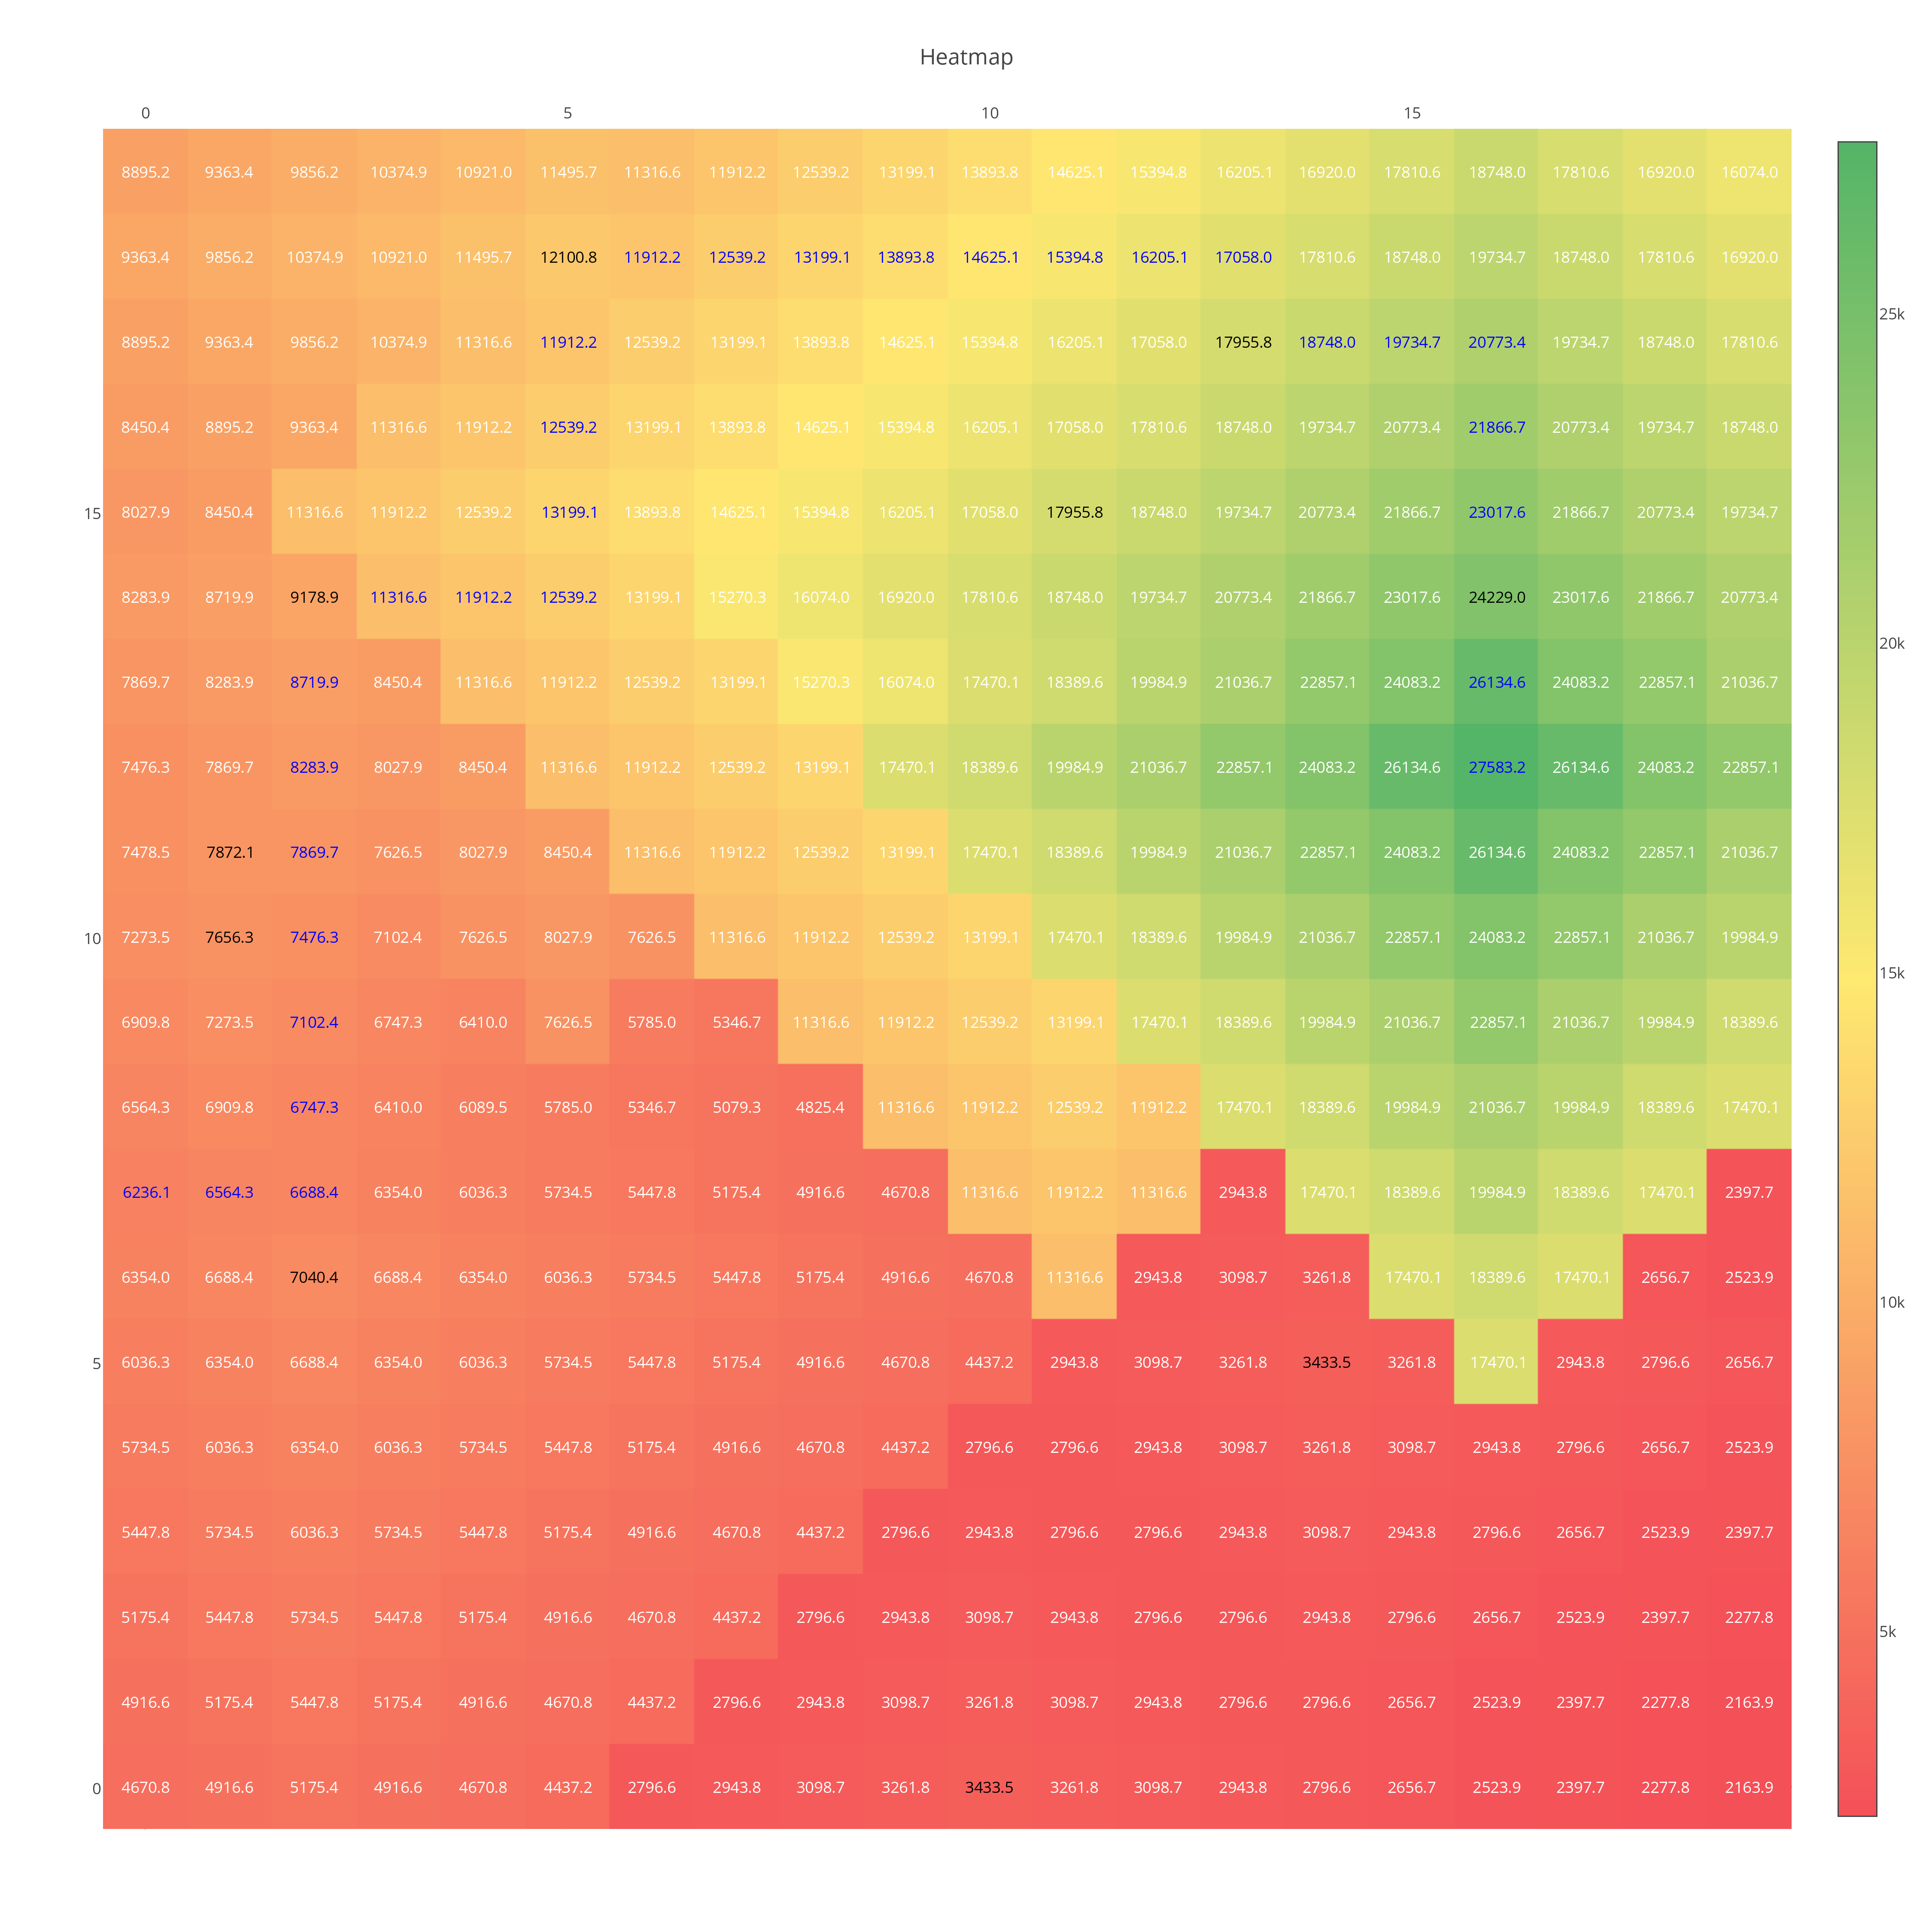
\includegraphics[scale=0.24]{x7y0}
\end{center}
  \caption{Heatmap showing optimal path found from (7,0) to destination (12,16)}
\label{fig:x7y0}
\label{fig:onecol}
\end{figure}

% \begin{figure}[h]
% \begin{center}
% \includegraphics[scale=0.22]{dest911start019}
% \end{center}
%   \caption{Heatmap showing optimal path found from (0,19) to destination (9,11)}
% \label{fig:long}
% \label{fig:twocol}
% \end{figure}

\subsection{Optimality}
Not perfect. We can see from figure \ref{fig:x7y0}, that 

\subsection{Reachability}
Heatmap provides very good view of which is reachable, and it also highlights the limitation of the current state of implementation

\section{Discussions}
\subsection{Sensitivity to reward parameters}
-very sensitive to choice of reward function with respect to parameters
\subsection{Scalability}
Takes about 150 iterations
\subsection{Solves a bigger problem}

\subsection{Next Steps}
\begin{enumerate}
\item online computation
\item quicker calculation
\item differing states have diff transition costs
\item adding more reward functions to skew preferences (arrival time, traffic conditions)
\item infinite vs finite horizon
\item choice of discount factor
\item integrate with real data google maps
\end{enumerate}


\section{Conclusion}

dope

{\small
\bibliographystyle{ieee}
\bibliography{egbib}
}

% \pagebreak[4]
\section{Appendix: Blown Up Figures}
\begin{figure*}[h]
\begin{center}
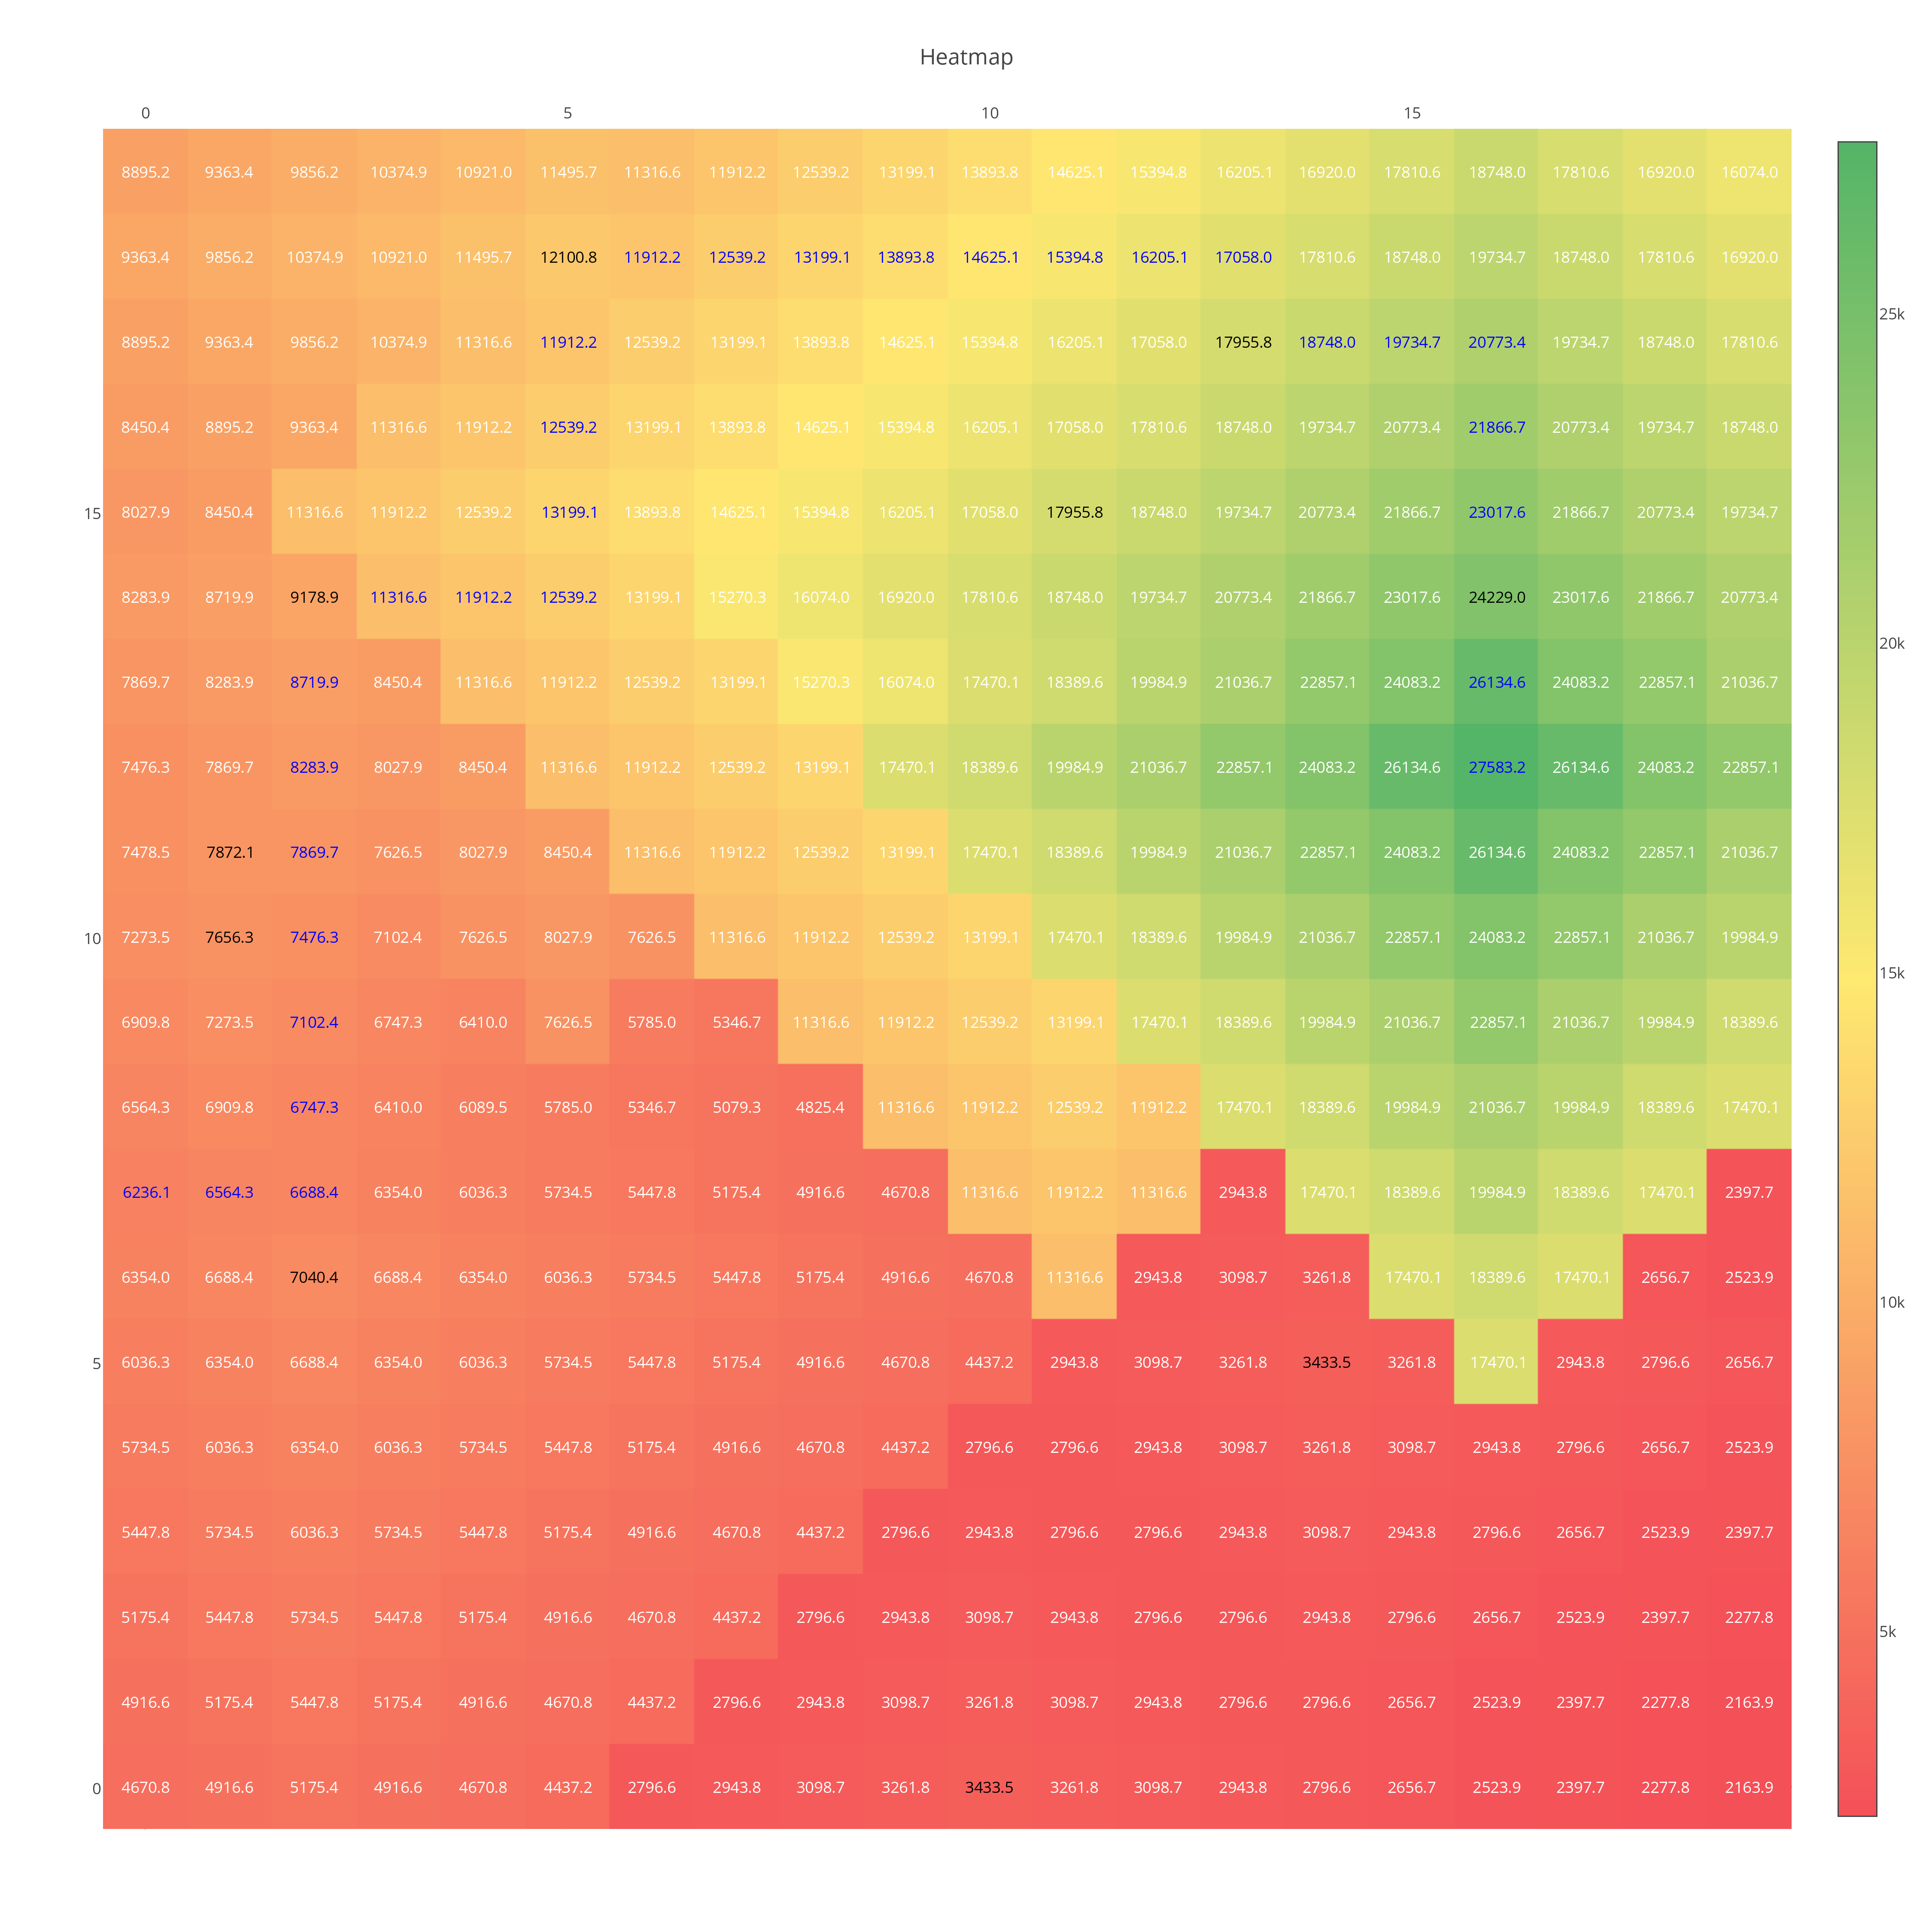
\includegraphics[scale=0.40]{x7y0}
\end{center}
   \caption{Heatmap showing optimal path found from (7,0) to dest (12,16)}
\label{fig:long}
\label{fig:onecol}
\end{figure*}

% \begin{figure}[h]
% \begin{center}
% \includegraphics[scale=0.4]{dest911start019}
% \end{center}
%   \caption{Heatmap showing optimal path found from (0,19) to (9,11)}
% \label{fig:long}
% \label{fig:twocol}
% \end{figure}

% \begin{figure}[h]
% \begin{center}
% 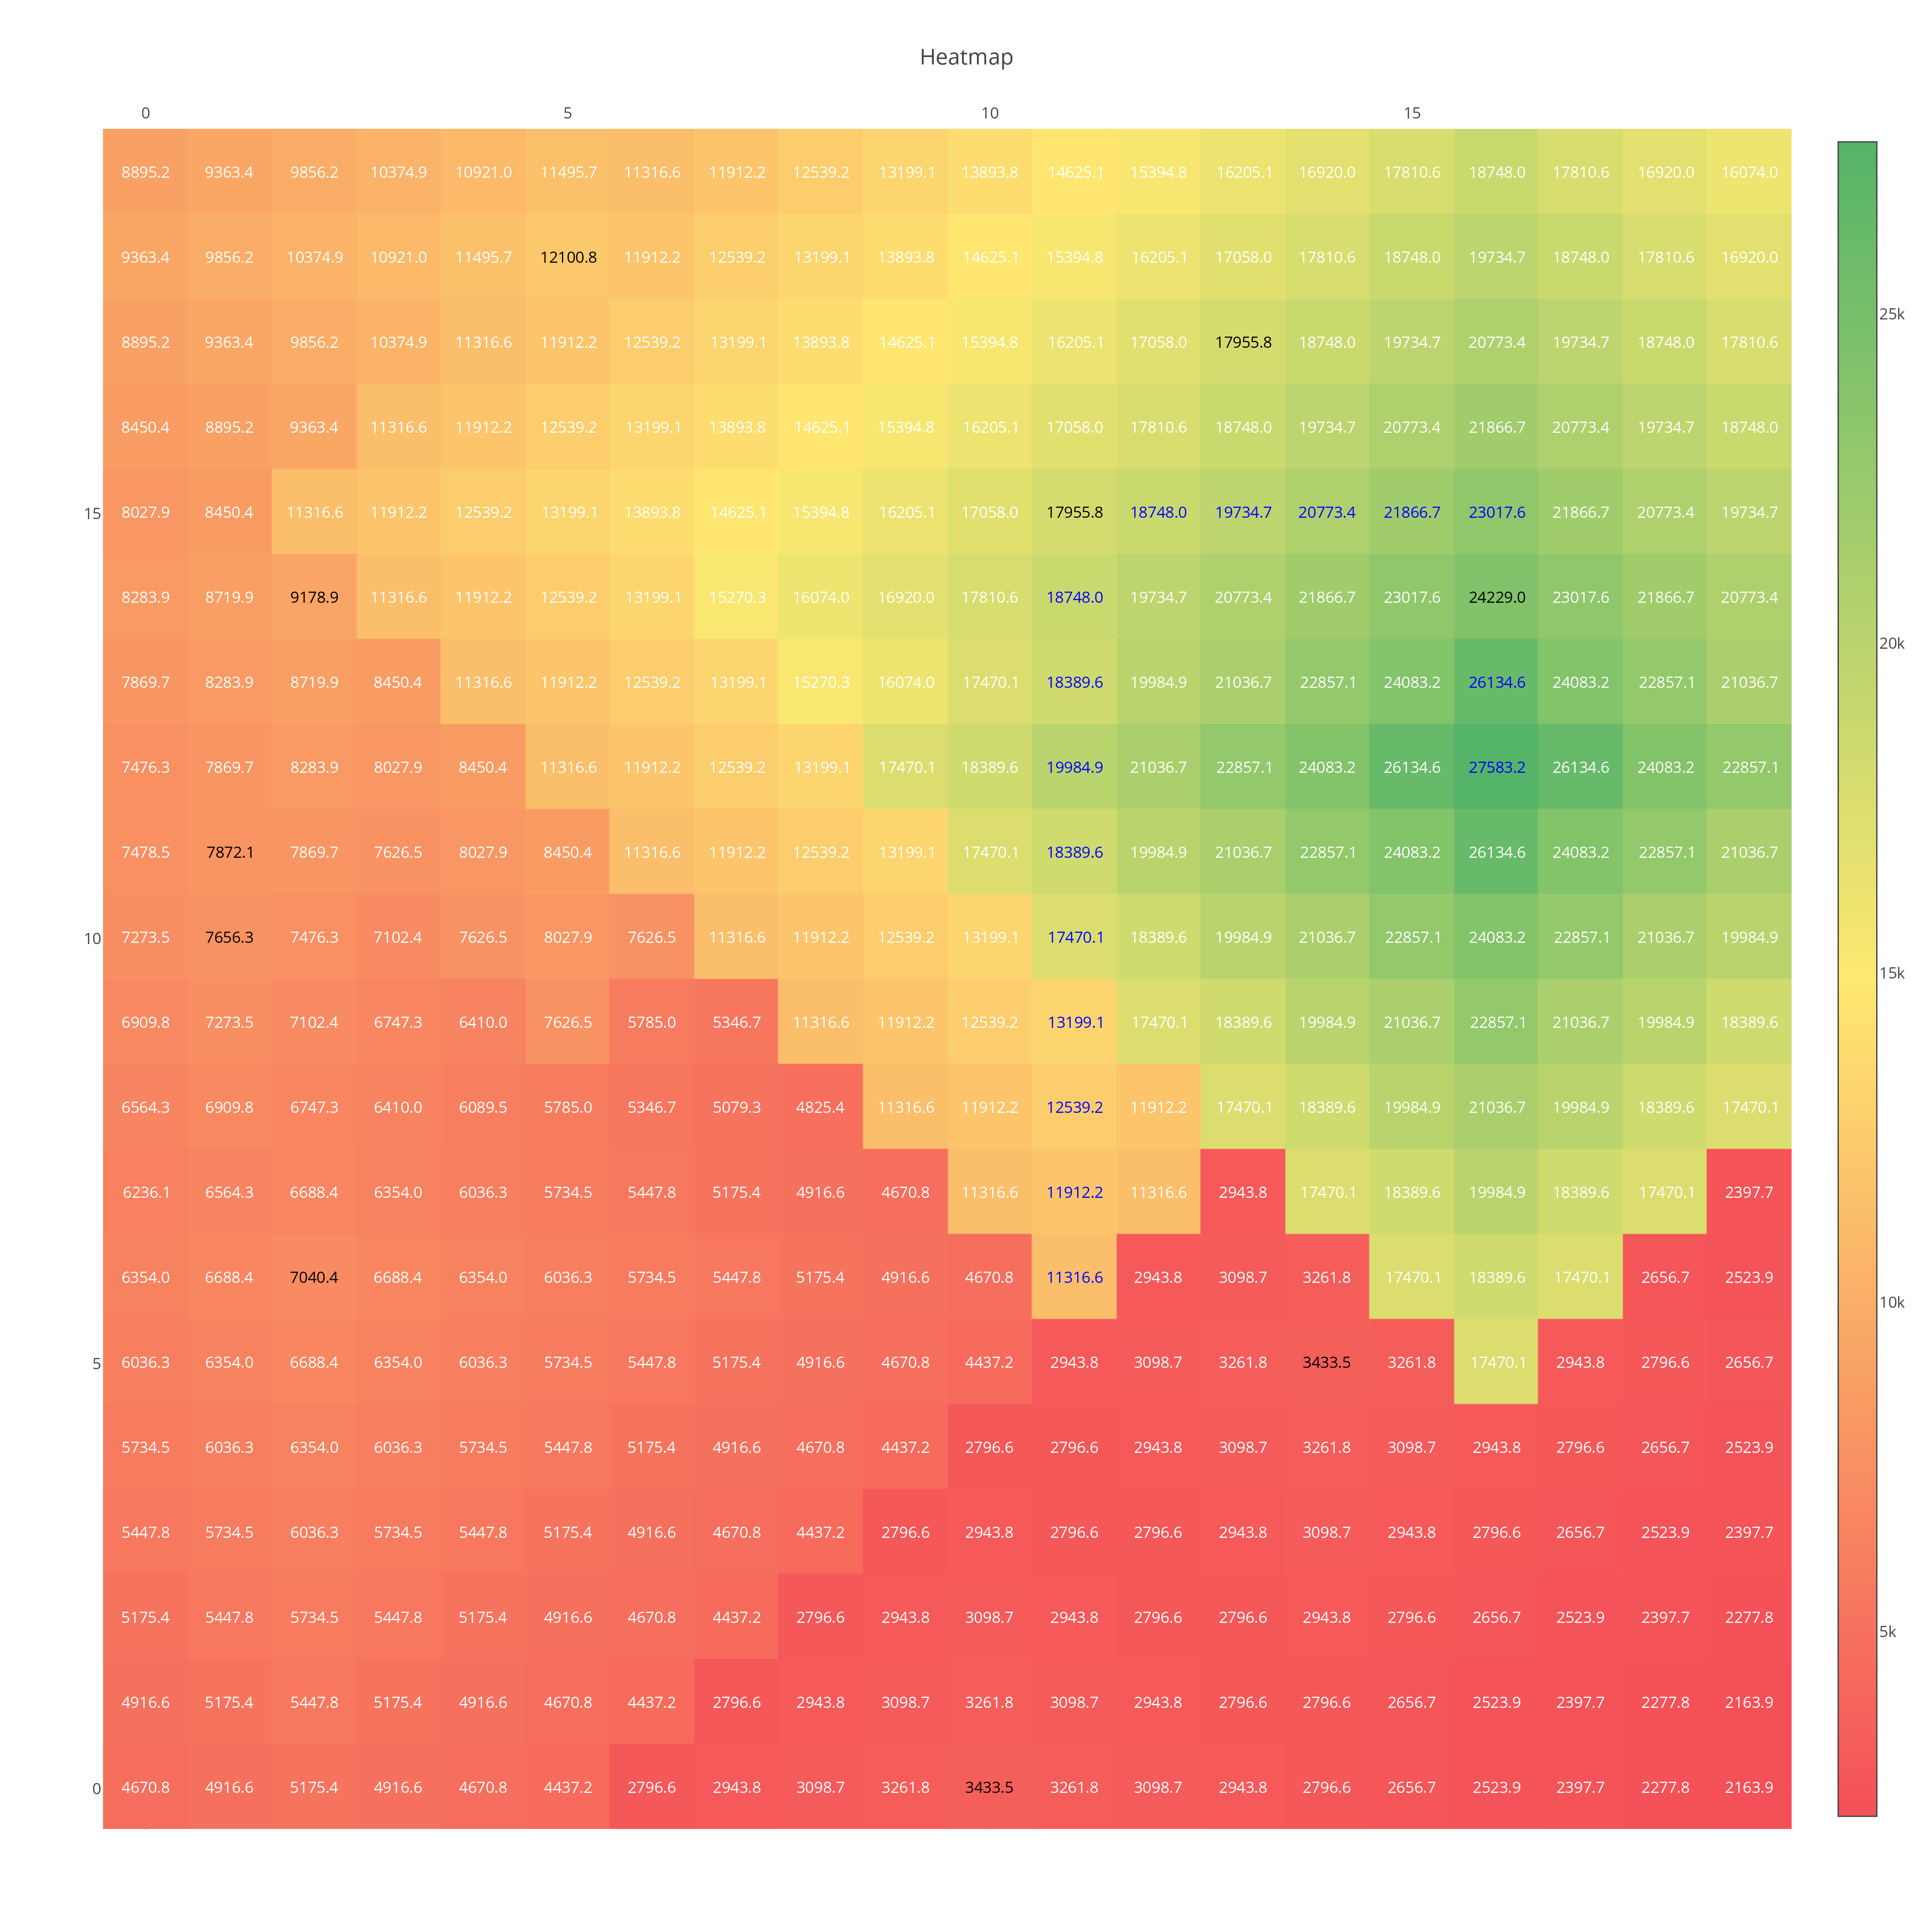
\includegraphics[scale=0.4]{x6y13}
% \end{center}
%   \caption{Heatmap showing optimal path found from (6,13
%   ) to (12,16)}
% \label{fig:long}
% \label{fig:twocol}
% \end{figure}


\end{document}
